\chapter{Parsovacie algoritmy}
Teoreticky je parsovanie vyriešený problém, ale je to druh problému, ktorý sa stále a znovu rieši. To znamená, že existuje veľa rôznych algoritmov, každý so silnými a slabými bodmi a akademici ich stále zlepšujú.\cite{tomassetti:parsing}

\section{Obecný prehľad}\label{parsing-alg-basics}
Metód parsovania existuje veľmi veľa. Pre praktické použitie však majú význam metódy, ktoré je možné rozdeliť do dvoch skupín:\cite{CVUT:program_language}
\begin{itemize}
\item Parsovanie \textbf{zhora dole (top down)} u ktorého sa parser najprv snaží identifikovať koreň parsovaného stromu, a potom postupuje dole cez podstromy až kým nenájde na listy stromu. Top down metóda je najrozšírenejšia zo spomenutých dvoch a existuje na ňu niekoľko úspešných algoritmov, ktoré ju uplatňujú. Tieto algoritmy najčastejšie využívajú funkcionalitu lookahead.
\item Parsovanie \textbf{zdola hore (bottom up)} u ktorej parser začína od najnižšej časti stromu, teda od listov a stúpa až do určenia koreňa stromu. 
\end{itemize}

Vezmime si pre príklad parsovací strom na obrázku \ref{fig:parseTreeExample}. 
\begin{figure}[H]
\begin{center}
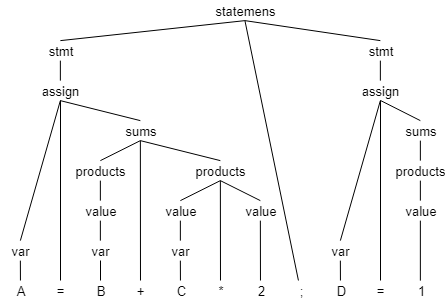
\includegraphics[width=7cm]{figures/parseTreeExample.png}
\caption{Typický parsovací strom pre výraz $A = B + C*2;  D = 1$}
\label{fig:parseTreeExample}
\end{center}
\end{figure}

Tento strom môže byť vygenerovaný oboma spomenutými metódami. Rozdiel bude iba v postupe jeho generovania. Na obrázkoch \ref{fig:parseTreeExampleTopDown} a \ref{fig:parseTreeExampleBottomUp} je možné vidieť poradie krokov ako postupovali oba typy parserov pri vytváraní uzlov stromu.

\begin{figure}[H]
  \centering
  \begin{minipage}[b]{0.45\textwidth}
    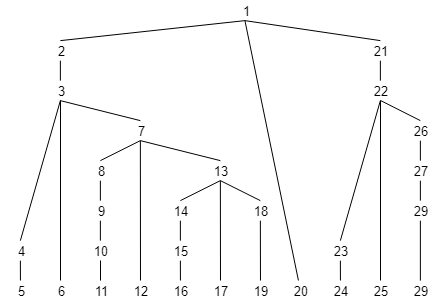
\includegraphics[width=\textwidth]{figures/parseTreeExampleTopDown.png}
    \caption{Postup generovania top down parseru}
    \label{fig:parseTreeExampleTopDown}
  \end{minipage}
  \hfill
  \begin{minipage}[b]{0.45\textwidth}
    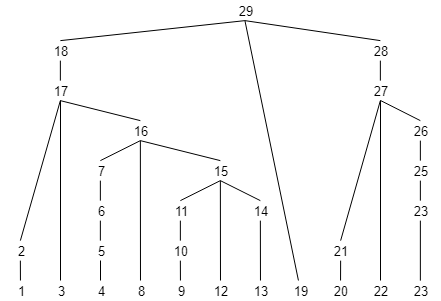
\includegraphics[width=\textwidth]{figures/parseTreeExampleBottomUp.png}
    \caption{Postup generovania bottom up parseru}
    \label{fig:parseTreeExampleBottomUp}
  \end{minipage}
\end{figure}

\textit{Top down} parsre sú jednoduchšie na poskladanie resp. implementáciu. Hoci sú \textit{Bottom up} parsere bežne považované za "výkonnejšie"{ }ako \textit{Top down} parsre, ich trieda jazykov ktorú dokážu rozoznať je rovnaká\cite{aho1972theory}. Tento výraz sa skôr vzťahuje k väčšej flexibilite v písaní gramatiky, kde oproti \textit{Top down} parserom nie je nutné dbať na pravidlá z ľavou rekurziou (viď kapitola \ref{ll_grammar}). Aktuálne je situácia vyváženejšia a to hlavne vďaka pokroku v stratégiách parsovania \textit{Top down} metódou. 

Nasledujúca tabuľka obsahuje súhrn hlavných vlastností existujúcich algoritmov a ich použitie\cite{tomassetti:parsing}.

\begin{longtable}{|p{2.5cm}|p{6cm}|p{5.5cm}|}
\hline
\textbf{Algoritmus}    & \textbf{Hlavné vlastnosti}    						& \textbf{Použtie} \\ \hline
\textbf{CYK} \cite{CYK} & V najhoršom prípade zložitosť O(n$^3$)\newline 
						Gramatika vyžaduje zápis CNF forme					& Špecifické problémy \\ \hline
                        
\textbf{Earley}
\cite{earley}		  & V najhoršom prípade zložitosť O(n$^3$), 
						no zvyčajne je lineárna\newline 
                        Dokáže spracovať všetky typy gramatík a jazykov		& Generátory parserov, ktoré musia 
                                                                              zvládať všetky typy gramatík  \\ \hline
                                                                              
  \textbf{LL} \cite{LL} & Jednoduchý na implementáciu \newline 
						 Nie až tak schopný ako väčšina algoritmov 
                         (nepodporuje ľavú rekurziu) \newline 
                         Historicky je najpopulárnejší						& Ručne vytvárané parsre a generátory 
                        													  parsrov, ktoré sú jednoduchšie na poskladanie  \\ \hline
                                                                              
\textbf{LR} \cite{LR}   & Náročné na implementáciu \newline 
						 Dokážu spracovať väčšinu gramatík, niektoré 
                         varianty dokonca všetky\newline 
                         Zvyčajne lineárna zložitosť, u dokonalejších 
                         variánt je zložitosť v najhoršom prípade O(n$^3$)		& Najvýkonnejšie generátory parserov \\ \hline
                         
\textbf{Packrat (PEG)}
\cite{Packrat}			& Lineárna zložitosť\newline 
						 Používa špeciálny formát zápisu gramatiky\newline 
                         Designovaný na parsovanie počítačových jazykov		& Jednoduché a zároveň výkonné parsre alebo 
                         													  generátory parserov pre počítačové jazyky \\ \hline         
\caption{Prehľad vlastností parsovacích algoritmov}
\label{my-label}
\end{longtable}

Väčšina parsovacích nástrojov pre bezkontextové gramatiky, ktoré sú schopné generovať parsre v programovacom jazyku Java\footnote{\url{https://en.wikipedia.org/wiki/Comparison_of_parser_generators}}, používa parsovacie algoritmy typu LL a LR. Z tohto dôvodu sa ďalej budeme venovať práve týmto typom algoritmov.

\subsection{Rekurzívny zostup}\label{recursive-descent}
Metóda rekurzívneho zostupu je technika parsovania, ktorá spočíva vo vytvorení samostatných procedúr na analýzu každého neterminálového symbolu. \cite{CVUT:program_language} Označenie poradia, v ktorom sa neterminálové prvky nachádzajúce sa na pravej strane použijú na získanie neterminálového symbolu na pravej strane pravidla sa volá \textit{odvodenie} alebo \textit{derivácia}. Existujú dve možnosti: \textbf{ľavá derivácia} a \textbf{pravá derivácia}. Prvá z nich znamená, že pravidlo sa uplatňuje zľava doprava, zatiaľ čo druhá presne naopak. 
\textbf{Note: možnosť pridať príklad ak je nutné}

Uplaňovanie derivácie sa vykonáva \textit{rekurzívne}. Pri top down parsovaní sa použije ľavá derivácia a pri parsovani bottom up pravá derivácia. Derivácia nemá žiadny vplyv na výsledný zparsovaný(derivčný) strom, ale má vplyv na použitý algoritmus.

\subsection{Lookahead a Backtracking}
Termíny lookahead a backtracking majú v parsovaní rovnaký význam ako v iných oblastiach informatiky. Lookahead označuje nasledujúcich počet prvkov, ktoré sa berú do úvahy pri rozhodovaní o aktuálnom prvku. Parser môže skontrolovať ďalší token a rozhodnúť sa, ktoré pravidlo sa má uplatniť. Takýmto parsrom sa tiež hovorí \textit{prediktívne} parsre \cite{haberman:parsing_demystified}.

Táto funkcionalita je dôležitá pre parsovacie algoritmy \textbf{LL}(viď kapitola \ref{LL}) a \textbf{LR}(viď kapitola \ref{LR}), pretože parsery pre jazyky, ktoré potrebujú iba jeden token lookahead sa jednoduchšie vytvárajú a sú rýchlejšie. Počet lookahead tokenov použitých v algoritme sa uvádza v zátvorkách za menom algoritmu (napr. LL(1), LR (k)). Použitie znaku hviezdy v zátvorkách naznačuje, že algoritmu môže skontrolovať nekonečné množstvo tokenov, aj keď to môže mať nepriaznivé účinky na výkon algoritmu.\cite{tomassetti:parsing}

Backtracking je technika algoritmu, ktorá spočíva v hľadaní riešenia komplexnejších problémov tým, že skúša riešenia čiastkových problémov, ktoré následne porovná a kontroluje to najsľubnejšie. Ak aktuálne kontrolované riešenie zlyhá, parser sa vráti späť na poslednú úspešne zanalyzovanú pozíciu a vyskúša iné riešenie.

\subsection{Lexikálna analýza pomocou DFA}
Ako bolo definované v kapitole \ref{DFA}, základným kameňom deterministického konečného automatu je množina stavov a prechodových funkcií. Tieto prechodové funkcie určujú, ako môže automat v závislosti na udalosti prechádzať z jedného stavu na iný. Pri použití v rámci lexikálnej analýzy, prijíma automat znak po znaku zo vstupného reťazca, až pokiaľ nedosiahne finálneho (akceptačného) stavu, čo znamená, že dokáže vytvoriť token \cite{roche1997finite}.

Lexikálna analýza spadá pod regulárne jazyky. Na základe definície \ref{def:regular_language} všetky regulárne jazyky sú prijímané deterministickým konečným automatom, a to je najzákladnejším dôvodom použitia DFA pre lexikálnu analýzu. Ďalším z dôvodov je možnosť spolupráce s online algoritmami.

Online algoritmus nepotrebuje na svoju prácu vedieť celý vstupný reťazec. Takéto algoritmy prijímajú sekvenciu znakov a vyhodnocujú ju priebežne \cite{karp1992line}. Pre lexer to znamená, že algoritmus dokáže rozpoznať token v momente keď vidí všetky znaky, ktoré ho definujú.

\section{LL parser}\label{LL}
Kategória \nom{LL}{Left-to-right read of the input, Leftmost derivation} parsrov spadá pod \textit{Top Down} parsre a ich názov vychádza z anglických názvov použitých techník (\textbf{L}eft-to-right read of the input, \textbf{L}eftmost derivation). To znamená, že číta vstupné symboly zľava doprava a snaží sa vytvoriť ľavú deriváciu. Tento algoritmus začína na štartovacom symbole a následne sa opakovane rozširuje do ľavého neterminálu, kým neskonštruuje cieľový reťazec. 

LL parsre sú založené na práci s parsovacou tabuľkou, pomocou ktorej sa rozhodujú, aké pravidlo gramatiky bude uplatnené. Využívajú techniku lookahead na sledovanie nasledujúcich tokenov, čím dokáže toto pravidlo presnejšie vybrať. LL parsre je ale možné ,a v praxi je aj častejšie využívané, implementovať pomocou rekurzívneho zostupu.

Koncept LL parserov sa nevzťahuje na žiadny konkrétny algoritmus, ale skôr na triedu parserov, ktoré sa definujú vo vzťahu  gramatikám. To znamená, že LL parser dokáže analyzovať LL gramatiku \cite{haberman:hard_parsing}.

Presná definícia LL gramatiky, sa ale vzťahuje ku počtu lookahead tokenov potrebných na jej zparsovanie. Na základe toho existuje niekoľko parsovacích algoritmov pre LL parsre. Základné tri algoritmy sú:
\begin{itemize}
\item \textbf{LL(1)} algoritmus s lineárnou zložitosťou, ktorý používa jeden lookahead token 
\item \textbf{LL(k)} algoritmus taktiež z lineárnou zložitosťou, ktorý používa \textit{k} lookahead tokenov.
\item \textbf{LL(*)} algoritmus, ktorý môže použiť neobmedzené množstvo lookahead tokenov. Teoretická asymtotická zložitosť tohto algoritmu je $O(n^2)$, no v praxi väčšinou kontrolujú jeden až dva lookahead tokeny \cite{LL}.
\end{itemize}

\subsection{LL gramatika}\label{ll_grammar}
LL gramatiky sú často používané práve kvôli veľkej obľube LL parserov aj napriek závažnej nevýhode. LL gramatiky \textbf{nepodporujú ľavú rekurziu}, čo znamená, že gramatiky, ktoré ju obsahujú, musia byť upravené do ekvivalentnej podoby bez ľavej rekurzie aby mohli byť parsované pomocou LL parserov.

Tento problém má za následok miernu stratu produktivity a výkonu \cite{tomassetti:parsing}. Výkonu z toho dôvodu, že pokiaľ gramatike z ľavou rekurziou mohol stačiť jeden lookahead token, u transformovanej gramatiky sa tento počet môže navýšiť na dva až tri tokeny. Problém produktivity spočíva v tom, že autor gramatiky musí písať gramatiku špeciálnym spôsobom, čo vyžaduje viac času. Tieto problémy bohužiaľ jemne podkopávajú silu algoritmu.

Na vysporiadanie sa s problémom ľavej rekurzie existuje ešte druhá možnosť. Namiesto ručnej úpravy gramatiky je možné použiť algoritmy, ktoré dokážu gramatiku transformovať. Niektoré s nástrojov využívajúce LL parsovanie majú takúto možnosť v sebe implementovanú, no ak by si autor chcel napísať vlastný parser, musí sa s tým vysporiadať sám.

\subsection{Príklad práce LL parseru}
NOTE: ak je nutné, prípadne ak bude treba nahrabať strany môžem pridať

\section{LR parser}\label{LR}
Algoritmy postavené na \nom{LR}{Left-to-right read of the input, Rightmost derivation} parsovaní sú hlavným dôvodom úspechu parsovania pomocou \textit{Bottom Up} metódy. Aj napriek tomu, že písanie LR gramatík prináša väčšiu flexibilitu oproti tradičným LL(1) gramatikám, ich popularita je bohužiaľ nízka a to najmä z dôvodu, že konštrukcia LR parserov bola v minulosti veľmi náročná \cite{tomassetti:parsing}. Názov LR vychádza z anglických názvov použitých techník (\textbf{L}eft-to-right read of the input, \textbf{R}ightmost derivation).

LR parsre spadajú do kategórie tzv. \textit{shift-reduce} parserov, ktoré pracujú v dvoch krokoch:
\begin{itemize}
\item \textbf{Shift}: Prečíta jeden token zo vstupného reťazca. Z tohto tokenu sa stane nový parsovací strom s jedným uzlom.
\item \textbf{Reduce}: Tento krok sa aplikuje ak sa sa nájde pravidlo gramatiky vytvorené z aktuálnych parsovacích stromov. Aplikovaním pravidla sa dané stromy spoja do jedného stromu z novým koreňom.
\end{itemize}

Jednoducho povedané, \textit{shift} operácia číta vstupný reťazec a \textit{reduce} operácia vytvára finálnu podobu parsovacieho stromu. V LR parsroch sa rozhodovanie o \textit{shift} a \textit{reduce} operáciách zakladá na všetkom, čo už bolo zparsované, a nie iba na jednom, najvyššom symbole v zásobníku. LR parsre dokážu riešiť toto rozhodovanie konštantnou rýchlosťou, a to zhromaždením všetkých príslušných informácií o sparsovanom kontexte do jedného čísla nazývaného stav parseru. Pre každú gramatiku existuje pevný (konečný) počet takýchto stavov \cite{LR}.

LL a LR parsre vznikli približne v rovnakej dobe a preto majú veľa spoločných faktorov. Rovnako ako u LL parserov aj LR využíva technológiu lookahead a počet používaných lookahead tokenov sa značí rovnako. To znamená, že LR(k) parsovací algoritmus dokáže parsovať gramatiku, ktorá vyžaduje \textit{k} lookahead tokenov. LR gramatiky sú menej obmedzujúce, a preto silnejšie oproti LL gramatikám. Jednou obrovskou výhodou je práve \textbf{podpora ľavej rekurzie}.

LR parsre taktiež pracujú s tabuľkami, ale namiesto jednej potrebujú dva komplikovanejšie. 
\begin{itemize}
\item Prvá napovedá parseru, čo má robiť na základe aktuálne čítaného tokenu, aktuálneho stavu a možných lookahead tokenov.
\item Druhá rieši prechod medzi jednotlivými stavmi po každej akcii.
\end{itemize}

Z popísaných informácií je vidieť, že LR parsre sú dostatočne výkonne a majú lineárnu zložitosť. Aj napriek tomu boli používané menej ako LL parsre a to práve z dôvodu tabuliek, ktoré používa. Tie sa ručne veľmi tažko vytvárajú a pri zložitejších gramatikách môžu byť veľmi veľké. V dnešnej dobe už existujú nástroje na generovanie týchto tabuliek priamo z gramatiky, no ak by si užívateľ volil vlastný ručne písaný parser, radšej by volil cestu \textit{Top Down} metódy.

\subsection{Simple LR a Lookahead LR}
Na základe toho ako sú tabuľky pre LR parser vygenerované, existuje viacero typov analyzátorov ako napríklad:

\textbf{TODO: dopisat nejake info a dat pridat odkaz}

\begin{itemize}
\item \textbf{Lookahead LR (\textbf{\nom{LALR}{Lookahead LR}})}, vynájdený profesorom  Frankom DeRemerom v rámci jeho dizertačnej práce\cite{deremer1969practical}. V tejto práci ukázal, že LALR parser má väčšiu schopnosť rozpoznávať jazyky ako LR(0) parser, pričom vyžaduje rovnaký počet stavov pre jazyk rozpoznateľný oboma analyzátormi. To robí LALR parser pamäťovo efektívnou alternatívou k analyzátoru LR(1) pre jazyky, ktoré sú LALR.

\item \textbf{Simple LR (\nom{SLR}{Simple LR})}, ktorý vypočítava lookahead tokeny jednoduchou aproximačnou metódou založenou priamo na gramatike, pričom ignouje individuálne stavy a prechody parsera. Použitie SLR gramatiky zabezečí, že pri parsovaní nenastanú žiadne \textit{shift/reduce} alebo \textit{reduce/reduce} konflikty\cite{deremer1971simple}.
\end{itemize}

Použitím týchto alternatívnych LR parsrov sa stráca výkonnosť parsru oproti originálnemu LR parsru. Poradie podľa výkonnosti je následovne:
\begin{center}
 LR(1) > LALR(1) > SLR(1) > LR(0) \cite{grune2007parsing}
\end{center}

\subsection{Príklad práce LR parseru}
NOTE: ak je nutné, príadne ak bude treba nahrabat stray môžem pridať

Názvy SLR a LALR parsrov sú trochu zavádzajúce, nakoľko SLR nie je až tak jednoduchý a LALR nie je jediný, ktorý používa lookahead tokeny. Dá sa povedať ze SLR je jednoduchší a rozhodovanie LALR veľmi úzko súvisí na lookahead tokenoch. Podstata ich rozdielu je v tabuľkách, kde menia časti o tom, čo majú robiť a lookahead sety. Tieto úpravy prinášajú určité obmedzenia na gramatiky, ktoré sú schopné zparsovať \cite{tomassetti:parsing}.

SLR parser je veľmi obmedzujúci a v praxi sa až tak veľmi nepoužíva. Na druhú stranu LALR parser dokáže spracovať väčšinu praktických gramatík a preto je široko používaný.

\section{Teória proti praxi}
Teória LL a LR parsovania je stará už viac ako 50 rokov. Prvá písomná zmienka o LR parsovaní \cite{LR} bola zverejnená v roku 1965. Od tej doby vzniklo obrovské množstvo  článkov o parsovaní a teórie jazykov, v ktorých akademici skúmali matematické rozmery parsovania. Aj napriek tomu sa v posledných rokoch objavujú nové a dôležité výsledky, čomu nasvedčuje aj prieskum spísaný v knihe \textit{Parsing Techniques: A Practical Guide} \cite{grune2007parsing} z roku 2007, ktorej bibliografia obsahuje viac ako 1700 citovaných článkov! \cite{haberman:hard_parsing}

Je bezpečné povedať, že základné LL a LR parsre sa ukázali ako veľmi nepostačujúce pre prípady používania v reálnom svete. Mnohé gramatiky, ktoré by boli prirodzene napísané pre tieto prípady, nie sú LL alebo LR, no stále existujú možnosti na ich rozšírenie, pomocou ktorých si dokážu zachovať svoje silné stránky. Dva najobľúbenejšie parsovacie nástroje založené na LL a LR (ANTLR a Bison) rozširujú algoritmy LL a LR rôznymi spôsobmi, pričom pridávajú funkcie ako prednosť operátora, syntaktické / sémantické predikáty, možnosť bactrackingu a generalizované parsovanie.

Dokonca aj tieto existujúce nástroje, nie sú stopercentne dokonalé a je nutné aby sa stále vyvíjali aj v rámci použitia, hlásenia chýb, lepšej vizualizácie, lepšej integrácie z programovacími jazykmi atď. Napríklad ANTLR v4 úplne prepracoval svoj analytický algoritmus na zlepšenie jednoduchosti použitia oproti predchádzajúcej verzie. Algoritmus predstavil pod názvom \textbf{\nom{ALL}{Adaptive LL}(*)}\cite{ALL} v roku 2014. Bison experimentuje s algoritmom \textbf{IELR} \cite{IELR}, čo je alternatíva k LALR, ktorá bola zverejnená v roku 2008 a má za cieľ rozšíriť počet gramatík, ktoré môže prijímať a parsovať efektívne.

\subsection{ANTLR alebo Bison?}
ANTLR a Bison sú nástroje na generovanie parserov, ktoré dokážu parsovať bezkontextové gramatiky. Najväčším rozdielom medzi nimi je konkrétny typ gramatiky, ktorú parsujú. Zatiaľ čo Bison parsuje LALR gramatiky (Bottom Up) ANTLR parsuje LL gramatiky (Top Down). 

Čo sa týka týchto gramatík, každá má svoje výhody a nevýhody. ANTLR v4 sa ale dokázal čiastočne zbaviť jednej závažnej nevýhody v LL gramatikách. Ako už bolo spomenuté LL gramatiky nepodporujú pravidlá s ľavou rekurziou. ANTLR v4 si však počas generovania parseru dokáže upraviť poskytnutú gramatiku a zbaviť sa \textit{priamych ľavých rekurzií} \cite{ALL}.

Bison generuje parsre, ktorých práca je založená na tabuľkách \cite{IELR}. Logika parsovania je teda uložená práve v týchto tabuľkách a nie priamo v kóde parseru. Z toho vyplýva, že parser má aj pre relatívne zložité jazyky malú stopu kódu. Na rozdiel od toho, ANTLR generuje parser s rekurzívnym zostupom. U takýchto parserov je každé pravidlo gramatiky reprezentované funkciou v kóde parseru. Z toho logicky vyplýva, že tieto parsre budú mať veľmi veľkú stopu kódu. Ako príklad uvediem parser vygenerovaný pre gramatiku MySQL obsahuje viac ako 58 000 riadkov kódu. Výhodou tohto prístupu je jednoduchšie pochopenie práce parseru a prípadne debugovanie. Taktiež parsre s rekurzívnym zostupom sú typicky rýchlejšie ako tie, ktoré využívajú na svoju prácu tabuľky. 

V neposlednom rade ďalšou výhodou pre ANTLR je grafický nástroj nazvaný \textit{ANTLRworks}\footnote{\url{http://www.antlr.org/tools.html}}. Tento nástroj je dostupný ako plugin do vývojových prostredí Intellij, NetBeans, Eclipse, Visual Studio Code, a jEdit. Počas toho ako užívateľ zadáva reťazec, ktorý chce zparsovať, tento nástroj vizualizuje parsovací strom a základe gramatických pravidiel a ak objavý konflikt, oznámi užívateľovi, čo ho spôsobilo. Súčasťou tohto nástroja je aj možnosť profilovania, ktorý vám pomôže pochopiť, ktoré rozhodnutia vo vašej gramatike sú komplikované alebo drahé.

ANTLR v4 je aktuálne z týchto dvoch nástrojov ten lepší najmä vďaka jeho novo vyvinutom algoritme ALL(*), ktorého teoretická zložitosť je $O(n^4)$, no na gramatikách používaných v praxi pracuje \textbf{lineárne} \cite{ALL}.

